\section{方法}
有别于其他类型的检测问题,如车牌检测和人脸检测,二维码检测有其独特的检测特征——二维码的编码特征。\\
二维码在设计过程中引入的定位模块,修正模块,对齐模块等编码模块都有助于快速准确地检测到二维码的位置。
基于二维码的编码特征,我们实现了两个二维码检测的方法,第一个相对简单直接,第二个针对复杂摄像环境下,对第一个方法做了改进。

\subsection{第一种方法:基础方法}
之所以称为基础方法,是因为这个方法直接利用二维码的编码特征,目的是为了从一幅简单的图片中定位二维码的位置。\\
基础方法的检测步骤如图\ref{fig:basic}所示。

\begin{figure}[h]
\centering
\includegraphics[width=0.9\linewidth]{../../../presentation/basic}
\caption[steps]{基础方法的检测步骤}
\label{fig:basic}
\end{figure}

\subsubsection{转换成灰度图}
为了减小计算量,一般将彩色图像转换成灰度图像。灰度图像与彩色图像一样反映整幅图像的整体和局部的色度和亮度等级的分布和特征。\\
图像的灰度化处理可以用两种方法来实现:(1).以每个像素点的R,G,B三个分量的平均值作为该点的灰度值。(2).根据YUV(亮度,色度,色温)颜色空间和RGB空间的对应关系进行转换,其中Y分量的物理意义是亮度,可以代表图像的灰度等级。利用公式\ref{yuv}可以将彩色图像转换成灰度图像,灰度级别为256,灰度图像中的像素为0~255的亮度值。
\begin{equation}\label{yuv}
Gray = 0.299 * R + 0.5866 * G + 0.1145 * B
\end{equation}
实验采用第二种方法来灰度化原始图像。

\subsubsection{高斯模糊}
对于灰度化的图像,我们采用高斯模糊来去除图像中的噪声,方便之后的轮廓检测。
高斯滤波算法中,分布不为零的像素组成的卷积矩阵与原始图像做变换。
每个像素的值都是周围相邻像素值的加权平均。
原始像素的值有最大的高斯分布值,所以有最大的权重,相邻像素随着距离原始像素越来越远,其权重也越来越小。
这样进行模糊处理比其它的均衡模糊滤波器更高地保留了边缘效果,这样就有利于我们之后的轮廓检测。\\
高斯模糊之后的图像如图\ref{fig:blured}(b)所示。
\begin{figure}[h]
\centering
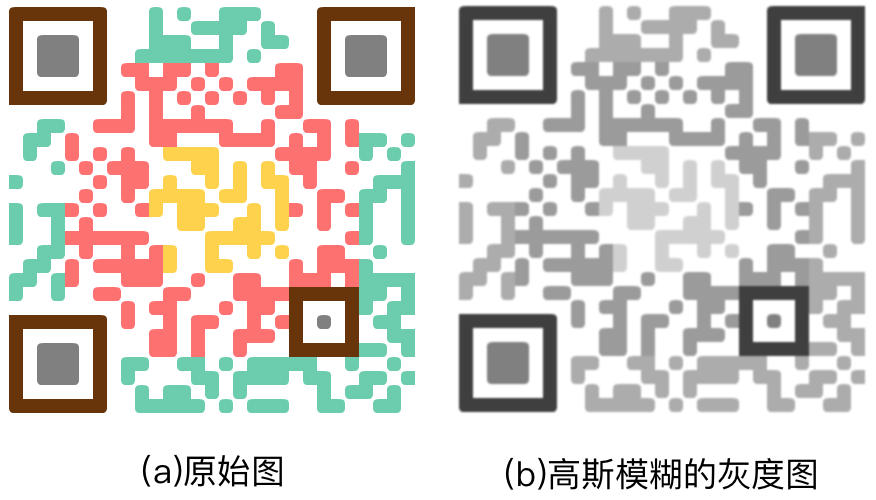
\includegraphics[width=0.9\linewidth]{blured}
\caption[blured]{QR码的原始图和模糊灰度图}
\label{fig:blured}
\end{figure}


\subsection{第二种方法:改进方法}
